\chapter{Contexte}
\section{Introduction}
    \subsection{Généralités}
        \subsubsection{Importance des données géotechiques en Haïti}
          \par
Avant d’investir des millions de dollars et des centaines d’heures pour 
construire un bâtiment, les propriétaires fonciers doivent savoir si le 
plancher peut supporter le bâtiment en question. Un sous-sol mou et 
rempli d'air peut conduire à un dépôt plus fort que souhaité, ce qui 
conduit à des fissures prématurées dans tout le bâtiment.
\par
De ce fait, le plus sage est de recourir au préalable à des études de sol.   
Malgré la valeur que peut coûter de telles études, que ce soit en termes
économique et/ou temporel, les caractéristiques d’un sol restent une
information essentielle à bien des égards. De ce fait, des études sont 
réalisées lors de la construction de grandes infrastructures ou de routes. 

        \subsubsection{Gestion des données géotechiques en Haïti}
            \par
Les outils papiers utilisés pour le moment sont très vulnérable à des
catastrophes comme des incendies ou des tremblement de terre. D'autres
part, lorsqu'ils sont numérisé, les fiches référencement, contenant les
informations relatives au dossier, sont souvent stockés sur supports
dur. La perte des documents de référence entraînerait un travail
colossal pour le recouvrement des informations relatives à chaque 
dossier.
\par
Diverses instances séparées détiennent des données recueillies au cours
de leurs études respectives. En effet, la sensibilité et l’importance de
ces dernières exigent l’existence de responsables dédiés à cette fin. 
Ainsi, lorsqu’un particulier a besoin de faire des études de sols, il 
fait appel à des instances clés capable de les prendre en charge. 
Parmi celles accessibles dans le pays, les plus contactées restent :
\begin{itemize}
    \item \textbf{URGéo}
    L'Unité de Recherche en Géosciences a pour mission de mener des
    recherches dans les domaines des géosciences où elle a les capacités
    pour le faire.Cela implique une bonne compréhension des différentes 
    problématiques liés au sol et au sous-sol et la proposition de moyens
    de mitigations adaptées à la réalité haïtienne.
    \cite{mission_urgeo}
    \\
    Pour le moment, l’URGéo constitue l’une des rares unités de recherches
    dédiée aux géosciences dans le pays. Ces chercheurs prennent part à de
    grandes réunions savantes et scientifiques en Amérique du Nord, en 
    Europe et dans les Caraïbes.
    \item \textbf{BME}
    Le Bureau des Mines et de l’Energie (BME) est un organisme autonome créé en 
    1986 fonctionnant sous la tutelle du Ministre des Travaux Publics, Transports 
    et Communications (MTPTC). Sa mission principale est de promouvoir la recherche
    et l'exploitation des ressources minérales et énergétiques d'Haíti ainsi que les 
    techniques appropriées y relative.
    \item \textbf{SICOD}
    La  Société d’Ingénierie Constructions et d’Orientations Diverses (SICOD),
    fondée en 2011, est une société haïtienne en noms collectifs qui évolue dans 
    les domaines d’ingénierie géotechnique et de constructions.
    Il s'adonnent aux prélèvements des données des essais de laboratoire, des 
    interprétations systématiques et aux recommandations techniques. 
    Ils apportent leur support technique aux maîtres d'ouvrages dans la réalisation 
    de leur chantier tout en observant les critères techniques de l'art.
    \item \textbf{LNBTP}
    Le LNBTP est une institution publique à gestion autonome chargée du contrôle de
    la qualité des infrastructures en construction dans le pays. Il s'occupe 
    aussi des études géotechniques, des recherches appliquées sur les matériaux de 
    construction et de la promotion des normes en matière de génie civil.
    \item \textbf{Géothechsol}
    Géothechsol est un Bureau d’Etudes en Ingénierie Géo\-technique et Environnemental
    ainsi qu’en formulation de béton et ses essais mécaniques et physiques, qui s’est
    fixé pour objectif de vous apporter une réponse sérieuse et de qualité, adaptée à 
    vos besoins dans le respect de vos contraintes. Ce bureau axe ses travaux sur les
     essais géotechniques et des sondages.
\end{itemize}   

\par
En général ces entreprises s'impliquent dans la construction et la recherche. 
Leur travail consiste à effectuer une reconnaissance/étude géotechnique des sites et
des échantillons  sont sélectionnés pour des analyses au laboratoire.
\par
Depuis plusieurs années ils se sont fait remarquer, notamment dans
l'étude des sols avant la construction de grands bâtiments. Ils sont aussi impliqués
dans la réalisation des ponts et des routes sur le territoire
haitiens. 

    \subsection{Problématique}
    \textbf{Comment arriver à gérer de façon optimale les données géo\-techiques 
    en Haïti et mutualiser les données sur le sous-sol accumulées par différents 
    organismes ?}
    \subsection{Panorama du projet}
        Avant d'entrer d'emblée dans le vif du sujet, nous aborderons 
d'abord l'état de l'art. Cette phase va nous permettre de capitaliser le 
savoir et le savoir-faire existants, et de ne pas refaire des expériences 
qui auraient déjà été faites et dont les conclusions ont déjà été validées 
par des pairs.
\par
Par la suite, on se penchera sur les différents éléments de réponse que l'on 
pourrait apporter au problème confronté.
Enfin nous metterons l'emphase sur l'implémentation des diverses solutions 
que l'on propose.


\section{Étude de l'existant}
    \subsection{Les BDD géotechniques dans le monde}
        \paragraph{}
Un système de gestion des informations géotechniques s'avère incontournable
dans un environnement de géoscience. Beaucoup d'universités et d'entreprises 
privées ainsi que l'état dans certains pays à travers le monde se sont déjà 
penchés sur la question. 
\paragraph{}
Les résutats divergent sur quelques détails à propos des technologies utilisées mais 
l'objectif est généralement le même: 
constituer une base de données renseignée regroupant tous les points (sondages, essais
in situ ou en laboratoire) améliorant la connaissance des caractéristiques géomécaniques des
formations d'une zone.
Par exemple, dans les Caraïbes, plus précisement sur l'Ile de Cayenne, un tel système a permis
de mieux appréhender les types de problèmes
spécifiques au site, et donc de mieux dimensionner les campagnes de reconnaissance
géotechniques, aussi bien sur le plan technique que financier
\cite{Cayenne}.
\par
L'une des faiblesses de certains projets est l'utilisation des outils de Microsoft
qui ne semblent pas assez 
adéquats. Ils sont trop génériques, ce qui empêche un stockage intelligent des données géotechniques
\cite{antoljak2012subsurface}.

%......................

\paragraph{}D'autres se basent de pŕeférence sur la Conception d'une architecture d'information 
géotechnique à l'aide de services Web
\cite{zimmermann2003design}.
Cette architecture d'information a été implémentée à Los Angeles afin de permettre les échanges 
d'informations géotechniques accessibles pour tous. Les avantages apportés par une telle 
application pourraient tant se sentir pour des études concernant les risques sismiques que pour 
une meilleure approche lors des estimations effectuées par des compagnies d'assurance. 

\paragraph{}
Au Canada, plusieurs projets identiques ont vu le jour, notemment l'élabora\-tion d'une base 
de données géoscientifiques dans le but d’aider à la finalisation de la 
cartographie des dépôts en surface et en subsurface
\cite{russell1996regional}.

%............................

\paragraph{}
En 2011, un séisme a frappé la région de Canterbury (Nouvelle-Zélande). Une base de données en ligne a été développée pour
la reconstruction de Christchurch à la suite du tremblement de terre:
La base de données géotechniques de Canterbury (CGD). Elle
a été conçu comme un référentiel consultable pour le partage d'informations géotechniques existantes et nouvelles
ainsi que des applications géotechniques de soutien pour les autorisations de construction. En mars
2015, la base de données contient plus de 18000 enregistrements d'essais de pénétration de cône, 4000 forages, 1000
piézomètres accompagnés de registres de surveillance des eaux souterraines, 6000 enregistrements de tests de laboratoire
plus d'autres données. 

\par
Le CGD a été conçu comme un référentiel consultable pour les informations géotechniques existantes et nouvelles
ainsi que des applications géotechniques de soutien pour les autorisations de construction et de ressources. Tandis que
les données sont principalement utilisées pour la conception géotechnique de l'amélioration du sol, la fondation du bâtiment
réparations, fondations de nouveaux bâtiments et conception géotechnique pour les réparations d'infrastructures, il peut
également être utilisé à des fins plus stratégiques telles que l'aide à la récupération pour de futurs
catastrophes naturelles, augmentation de la résilience d'autres régions de la Nouvelle-Zélande.
\cite{scott2015benefits}


\begin{figure}[t]
\centering
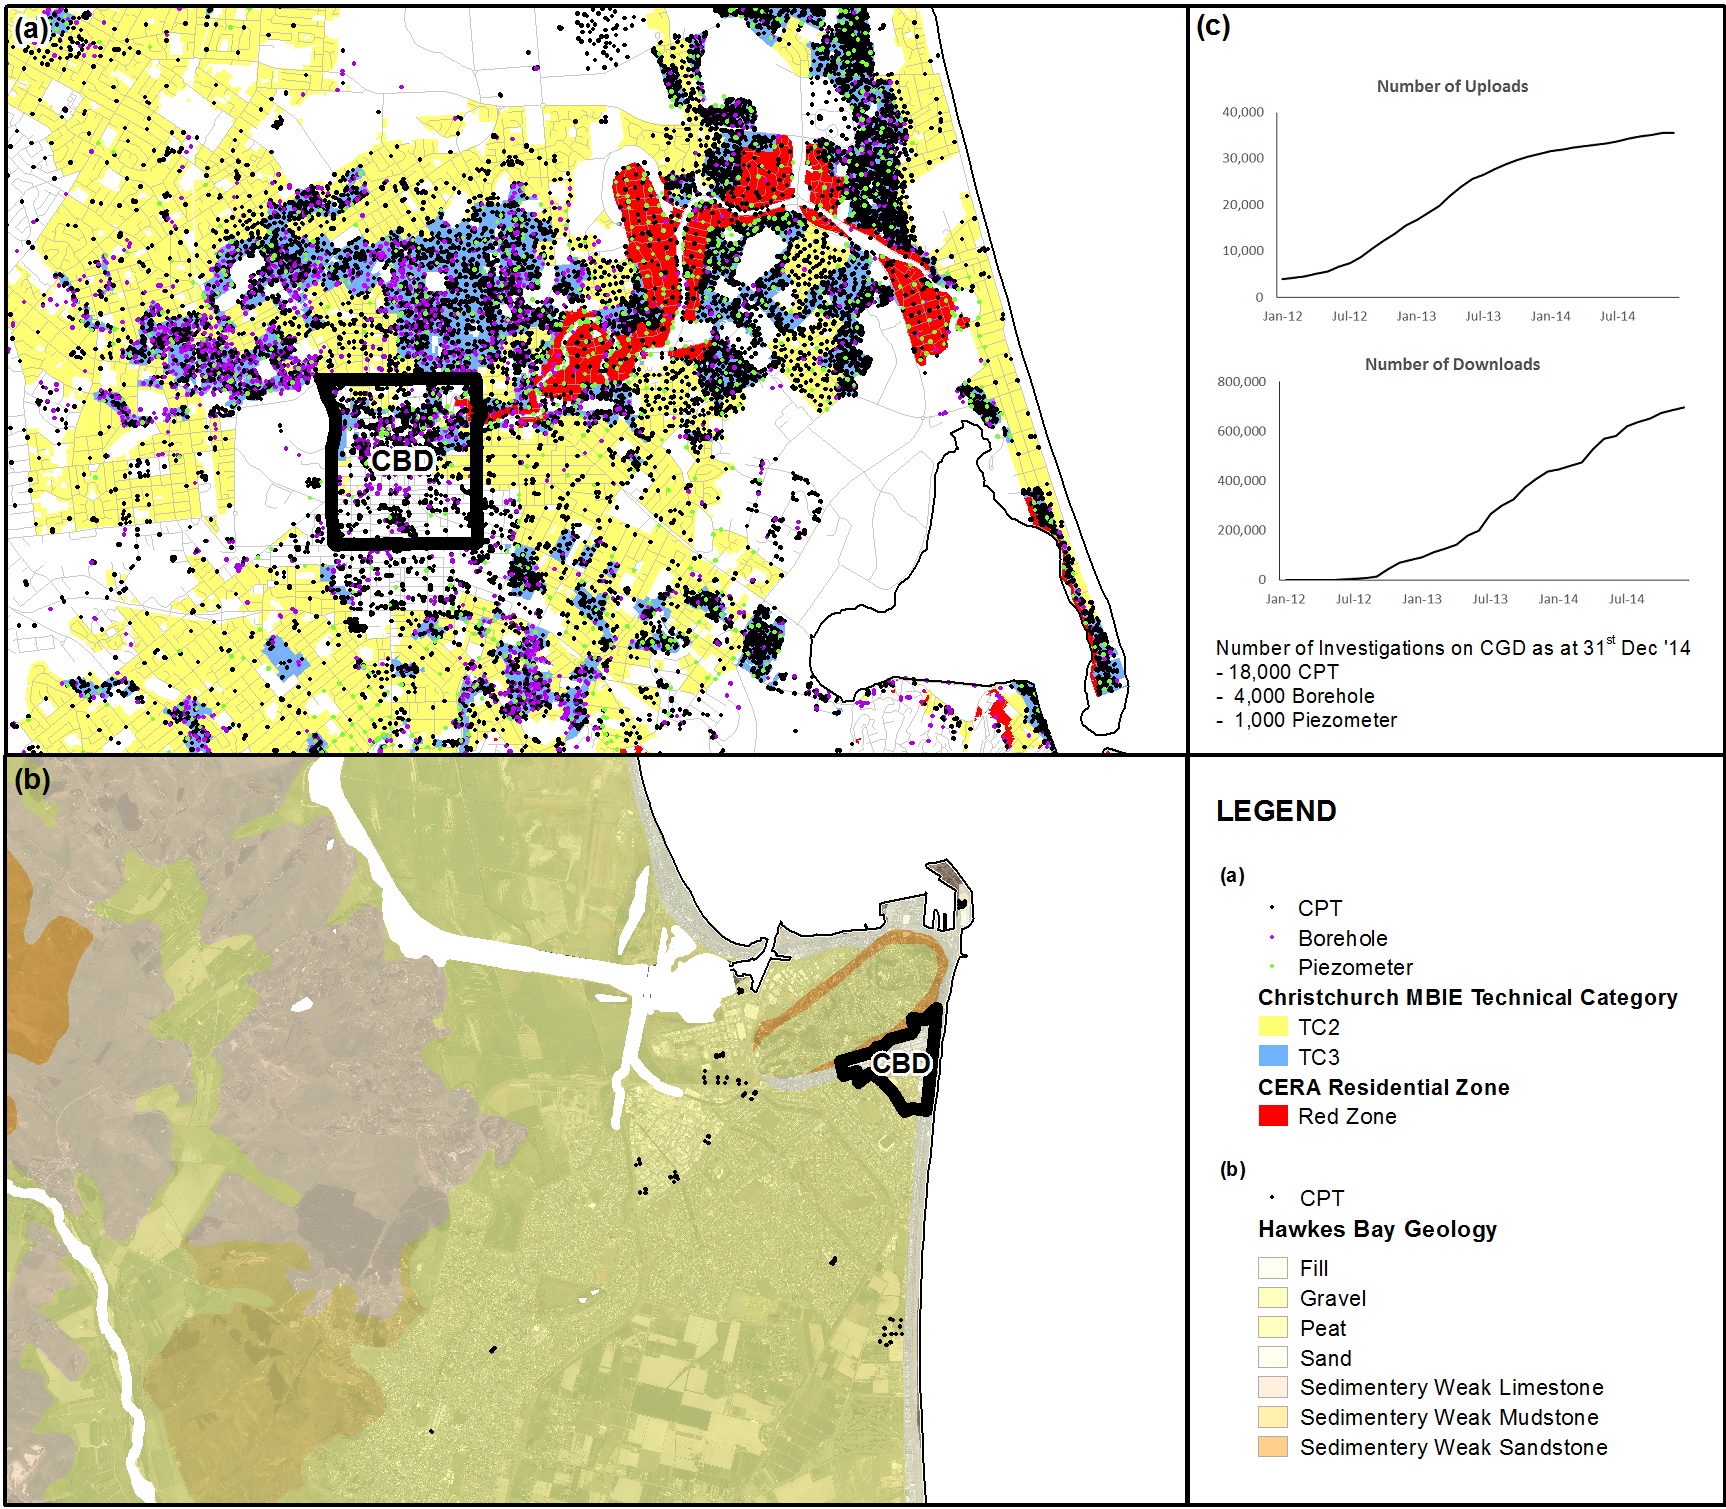
\includegraphics[width=1\textwidth]{cgd.png}
\caption{Visualisation des résultats de la base de données de Canterbury.}
\end{figure}

%............................

\paragraph{}
L'Afrique ne fait pas exception à la liste des multiples endroits ayant adopté l'idée
de concevoir une base do données géotechniques.
Par exemple, celle de la ville de Tunis (Tunisie) est orientée vers la cartographie géotechnique.
\par
Le modèle choisi a permis, après une analyse
pré1iminaire très importante, une description globale et
totale de toutes les données géologiques et géotechniques collectées sur le site de Tunis. I1
assure, de plus, une indépendance physique et logique, un partage des données (une même donnée accessible  
par plusieurs programmes), une non redondance des données, une non codification des
données géologiques, une grande facilité des relations
entre fichiers indépendants, une intégrité (validité)
totale des données. 
\textit{S'y ajoutent une souplesse remarquable d'interrogation de TUNIS-DATA-BANK
assurée par l'emploi d'un langage d'interrogation spécifique et l'utilisation des opérateurs et des connecteurs
logiques, une automatisation totale des tâches de la
phase de la manipulation de la base de données et une
sécurité totale des fichiers.}
\cite{tunis}

%..................

\paragraph{}
L’implémentation de tous ces SIG par des organismes internationaux résulte à des données considérées 
comme étant le système d’archivage officiel dans leur domaine de spécialité.
Le rythme de migration de ces données dans le SIG Web connait une croissance exponentielle. 
\par
Avec son mouvement vers le cloud et sur le Web, son intégration à l'information 
en temps réel via l'Internet des objets, le SIG est devenu une plateforme 
pertinente pour presque toutes les activités humaines - un système nerveux de 
la planète. Alors que notre pays est confronté au problèmes de gestion et de vulgarisation 
des données géotechiques, les SIG joueront un rôle de plus 
en plus important et 
fourniront un moyen de communiquer des solutions en utilisant le langage commun de 
la cartographie.
    \subsection{Avantages d'un Système de gestion des Informations Géotechniques}
        \paragraph{}
\textit{Un avantage d'un système de gestion de données géotechniques est 
la facilité avec laquelle les données 
peuvent être visualisées, filtrées et manipulées.
De plus, grâce aux règles métier, à la validation des données et aux 
processus de contrôle de qualité approfondis, le risque de trouver
des informations inexactes sont considérablement réduites. Une base de 
données correctement conçue ne nécessitera que les entrées de données
une fois, éliminant le besoin de ré-entrée et de reformatage. Une 
étude réalisée par Goldin et al.,
(2008) a montré qu'en moyenne 1,24\% des entrées de données dans Excel 
sont saisies de manière incorrecte; l'erreur alors
composés chaque fois que les données sont réintroduites. La mise en place 
«à entrée unique» d’une base de données bien conçue réduit les erreurs de 
transcription humaine, source majeure d’inexactitude pour les entreprises
traitant de grandes quantités de données géotechniques.}
\cite{keen2015development}
\paragraph{}
Étant donné que cet outil n'existe pas 
en Haïti, l'ampleur de ce projet fait donc surface.
D'où l'implémentation qui suit.

\section{Cheminement de la solution}
    \subsection{Implémentation d'une BDD géotechniques}
        \subsubsection{Numérisation des données}
            \par
Au cours de la première étape, des données seront recueillies à 
travers diverses instances partenaires, principalement l'URGéo. 
Enregistrées sous divers formats(papiers, CSV, PDF entre autres), 
ces informations seront par la suite normalisées puis numérisées. En 
effet, une structure uniforme devra être imposée afin de satisfaire la 
compréhension de tout particulier. Par exemple, MPOKO JWENN...
        \subsubsection{Intégration de ces données dans une BDD}
            \par
Évidemment, une simple numérisation ne changerait point grand chose 
si les données restent stockées sur des disques comme à l'ancienne. Ainsi, 
la normalisation ayant apporté un standard et une uniformité au sein des informations 
enregistrées, ces dernières pourront parfaitement être intégrées dans 
une base de données créée à cette fin. Une fois implémentée, cette 
base pourra héberger toutes les informations géotechniques relatives 
à une analyse effectuée par l'une des instances concernées. Plus 
explicitement, l'URGéo pourra enregistrer les résultats obtenus lors 
d'un forage, en alimentant la BDD tout en respectant les critères de 
standardisation.
\paragraph{}
Bien qu'efficace, cette BDD géotechniques reste un concept assez 
abstrait pour un concerné direct qui ne verra aucune différence 
entre ce nouveau format et les fichiers auxquels il était 
précédemment habitué.
    \subsection{Utilisation d'un SIG}
        \subsubsection{Connection de la carte d'Haïti et de la BDD}
            \par
Comme réalisé dans différents pays à travers le monde, la prochaine 
étape consistera à utiliser un Système d'Information Géographique (SIG) 
capable de faciliter l'interprétation scientifique de ces données. 
Les SIG permettent aux utilisateurs de créer leurs propres couches de cartes 
afin de résoudre des problèmes concrets. Ils ont également évolué ces dernières années pour 
devenir un moyen de partage de données et de collaboration, inspirant une 
vision qui devient aujourd’hui une réalité - une base de données qui 
couvre pratiquement tous les sujets; dans le cas présent, ce sera la géotechnique. 
Une fois le SIG lié à la base, tout intéressé pourra accéder aux informations 
enregistrées, dans un format plus conventionnel. Cela facilitera la visualisation des données. 
Dans le cadre de ce projet, il 
pourra trouver les résultats des tests effectuées au niveau d'une zone précise.
        \subsubsection{Utilisation de fonds de carte}
            \par
Une fois les informations accessibles, l'interprétation devient 
plus évidente; ce qui peut, pourtant, s'avérer insufisant. Par 
ailleurs, des images relatives au contexte recherché par le scientifique 
resteront inévitables. De ce fait, différents fonds de carte seront mis 
à la disposition de ce dernier, facilitant sa manipulation des données. 
L'ingénieur civil voulant faire des études en hydraulique pourra ainsi 
interprêter les données relatives à son domaine en sélectionnant son 
contexte personnel.
\paragraph{}
Désormais, tout particulier pourra accéder aux données de la BDD 
géotechniques en se référant à son domaine d'ètude. Néanmoins, tout 
autre action de sa part demandera l'intervention d'un expert en base 
de données.
    \subsection{Visualisation des données} 
        \subsubsection{Implémentation d'un UI intégrant un webmap}
            \par
Finalement, la dernière étape consistera à mettre à la disposition 
de nos utilisateurs finaux un interface adéquat et facilement 
accessible, leur permettant ainsi d'interagir avec la BDD. Grâce 
à cela, un administrateur pourra directement ajouter, afficher, modifier ou supprimer 
des informations sans avoir à contacter un expert en informatique.
Quant aux simples visiteurs, ils auront la possibilité de visualiter les données sur une carte. 
Ces données vont permettre aux utilisateurs(ingénieurs, étudiants, etc) de prendre des décisions, 
d’analyser des situations précises, ou encore de donner des alertes par rapport à des évènements précis.
\par
En effet, l'autonomie de tous les utilisateurs sans formation préliminaire 
traduira la performance de l'application. L'expérience utilisateur n'est pas anodin dans 
le développement d'un tel système.
        \subsubsection{Publication de l'interface}
            \par
Quelle serait l'utilité d'une application de cette envergure 
si sa portabilité n'était pas prise en compte ? - Aucune. Par 
conséquent, son déploiement dans le cloud relèvera d'un processus incontournable 
afin de la mettre à la disposition de tous les intéressés. Désormais, 
n'importe qui aura la possibilité d'accéder au portail web sans 
installation préalable. Néanmoins, pour une question de sécurité, 
certaines fomctionnalités exigeront à l'utilisateur/administrateur une authentification.
    \begin{figure}[t]
        \centering
        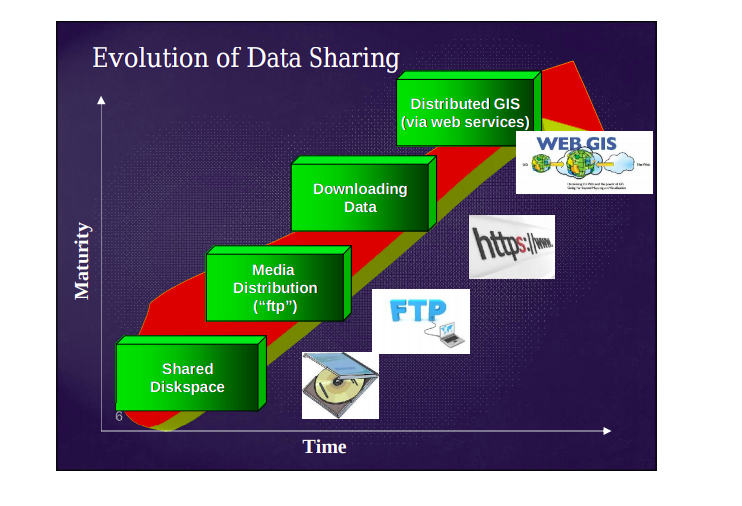
\includegraphics[width=1\textwidth]{images/evolution_projetGIS.png}
        \caption{Cheminement de la solution}
    \end{figure}

\section{Perspective de réalisation}
    \par
Étant plus que pragmatiques, nous ne nous limiterons pas à proposer 
uniquement une solution théorique. Nous mettrons la main à la pâte afin
de donner des résultats palpables et fonctionnels.
\par
Pour ce faire, nous définissons un cheminement, un ensemble d'étapes à 
respecter pour aboutir à un résultat optimal au moindre coût.
Ce cursus comprend cinq grandes étapes: 

\begin{itemize}
    \item \textbf{L'initialisation du projet: }
    Cette étape marque le début de notre long parcours et aura comme principaux
    objets la prise de connaissance du problème (dans le CDC) et l'identification des voeux
    l'URGéo.
    \item \textbf{Planification: }
    Tout grand projet digne de ce nom doit être planifié. C'est au cours de cette étape
    que létat de l'art sera traité pour prendre connaissance de l'existant et s'inspirer des travaux
    similaires déjà réalisés. Puis vient la phase de l'analyse, de l'évaluation des coûts du projet, 
    du choix  de l'architecture, des modèles,
    ainsi des technologies et des méthodes que l'on aura à utiliser.
    \item \textbf{Exécution: }
    L'essence de cette étape se trouve dans la réalisation même du projet, que ce soit en matière de base de 
    données ou de programmation.
    \item \textbf{Monitoring et contrôle: }
    Ici il s'agit d'effectuer des tests sur la qualité du produit final et et de vérifier si on a atteint le 
    résultat escompté. Notons que cette partie pourra se faire en parallèle avec l'éxécution, en faisant de 
    l'intégration continue.
    \item \textbf{Fermeture: }
    Enfin, on aboutit à la clôture du projet apres déploiement et une potentielle période de maintenance.


\end{itemize}  